% ============================================================
%  Swarm Auditor – Final Report
%  Author: Birkity Yishak
%  Date:   February 28, 2026
%  Course: 10 Academy — FDE Challenge Week 2
% ============================================================

\documentclass[11pt,a4paper]{article}

% ── Packages ────────────────────────────────────────────────
\usepackage[utf8]{inputenc}
\usepackage[T1]{fontenc}
\usepackage{lmodern}
\usepackage[margin=2.5cm]{geometry}
\usepackage{graphicx}
\usepackage{booktabs}
\usepackage{hyperref}
\usepackage{xcolor}
\usepackage{listings}
\usepackage{tikz}
\usetikzlibrary{arrows,shapes.geometric,calc}
\usepackage{enumitem}
\usepackage{amsmath}
\usepackage{fancyhdr}
\usepackage{titlesec}
\usepackage{caption}
\usepackage{float}

% ── Colours ─────────────────────────────────────────────────
\definecolor{codegreen}{rgb}{0,0.6,0}
\definecolor{codered}{rgb}{0.7,0,0}
\definecolor{codebg}{rgb}{0.97,0.97,0.97}
\definecolor{linkblue}{rgb}{0.04,0.28,0.56}

% ── Hyperlink style ─────────────────────────────────────────
\hypersetup{
    colorlinks=true,
    linkcolor=linkblue,
    urlcolor=linkblue,
    citecolor=linkblue,
}

% ── Listings style ──────────────────────────────────────────
\lstset{
    basicstyle=\ttfamily\small,
    backgroundcolor=\color{codebg},
    keywordstyle=\color{codered}\bfseries,
    commentstyle=\color{codegreen},
    frame=single,
    breaklines=true,
    columns=flexible,
    numbers=left,
    numberstyle=\tiny\color{gray},
    xleftmargin=1.5em,
}

% ── Header / Footer ────────────────────────────────────────
\pagestyle{fancy}
\fancyhf{}
\fancyhead[L]{\small Swarm Auditor: Final Report}
\fancyhead[R]{\small Birkity Yishak}
\fancyfoot[C]{\thepage}
\renewcommand{\headrulewidth}{0.4pt}

% ── Title ───────────────────────────────────────────────────
\title{%
    \vspace{-1cm}
    \textbf{Swarm Auditor: Final Report}\\[0.3cm]
    \large FDE Challenge Week 2: The Automaton Auditor\\[0.2cm]
    \normalsize 10 Academy
}
\author{
    Birkity Yishak\\
    \small \url{https://github.com/Birkity/automaton-auditor-fde-week2}
}
\date{February 28, 2026}

% ============================================================
\begin{document}
\maketitle
\thispagestyle{fancy}

% ────────────────────────────────────────────────────────────
\section{Executive Summary}
% ────────────────────────────────────────────────────────────

The \textbf{Swarm Auditor} is a deep LangGraph agent that audits Week~2 submissions
using a multi-layered ``Digital Courtroom'' architecture.  It evaluates code
repositories and PDF reports against a 10-dimension forensic rubric and produces
structured Markdown audit reports with per-criterion scores, judicial arguments,
dissent explanations, and remediation plans.

The system uses a \textbf{hybrid LLM architecture}: deterministic Python tools
form the backbone for forensic evidence and scoring, while three LLM models
(\texttt{deepseek-v3.1:671b-cloud} for heavy reasoning,
\texttt{qwen3-coder:480b-cloud} for structured judicial output, and
\texttt{Qwen2.5-VL-32B-Instruct} for multimodal vision) handle interpretation
and report polishing.  The system is \textbf{rubric-independent}: adding new
dimensions to \texttt{rubric.json} requires no code changes.

\begin{table}[H]
\centering
\caption{Key Metrics}
\begin{tabular}{@{}ll@{}}
\toprule
\textbf{Metric} & \textbf{Value} \\
\midrule
Graph Nodes            & 12 (including error handlers) \\
Conditional Edges      & 2 (\texttt{add\_conditional\_edges()}) \\
Parallel Fan-Out Layers & 2 (Detectives + Judges) \\
Rubric Dimensions      & 10 \\
Forensic Tools         & 12 (7 primary + 5 supplementary) \\
Test Count             & 221 across 10 test files \\
Self-Audit Score       & 3.9\,/\,5.0 \\
LangSmith Tracing      & Enabled \\
\bottomrule
\end{tabular}
\end{table}

\begin{table}[H]
\centering
\caption{Self-Audit Score Summary}
\begin{tabular}{@{}lc@{}}
\toprule
\textbf{Dimension} & \textbf{Score} \\
\midrule
State Management Rigor           & 5/5 \\
Graph Orchestration Architecture & 5/5 \\
Safe Tool Engineering            & 5/5 \\
Git Forensic Analysis            & 4/5 \\
Structured Output Enforcement    & 4/5 \\
Chief Justice Synthesis Engine   & 4/5 \\
Report Accuracy (Cross-Ref.)     & 4/5 \\
Judicial Nuance and Dialectics   & 3/5 \\
Theoretical Depth (Documentation)& 3/5 \\
Architectural Diagram Analysis   & 2/5 \\
\midrule
\textbf{Overall}                 & \textbf{3.9\,/\,5.0} \\
\bottomrule
\end{tabular}
\end{table}

% ────────────────────────────────────────────────────────────
\section{Architecture Deep Dive}
% ────────────────────────────────────────────────────────────

\subsection{System Overview}

The Swarm Auditor implements a three-layer pipeline modelled as a LangGraph
\texttt{StateGraph} with 12 nodes and 2 conditional edges.  The architecture
augments a deterministic detective layer and chief justice with optional LLM passes:

\begin{lstlisting}[language={},title={Pipeline Flow}]
START
  -> context_builder                   (loads rubric.json)
  -> [RepoInvestigator || DocAnalyst   (Hybrid: deterministic + deepseek LLM
     || VisionInspector]                fallback for unknown dimensions)
  -> evidence_aggregator                (post-process cross-refs)
  -> (conditional: has_evidence?)
      YES -> judge_dispatcher
             -> [Prosecutor || Defense  (LLM: qwen3-coder:480b-cloud
                || TechLead]             structured output via Pydantic)
             -> chief_justice            (Deterministic 5-rule scoring
                                         + deepseek LLM report polish)
             -> (conditional: report_valid?)
                 YES -> END
                 NO  -> report_fallback -> END
      NO  -> no_evidence_handler -> END
\end{lstlisting}

\subsection{Dialectical Synthesis}

The judicial layer implements \textbf{dialectical synthesis}, a reasoning pattern
where three adversarial personas analyse the same evidence from fundamentally
different philosophical positions:

\begin{description}[leftmargin=1.5cm,style=nextline]
    \item[Prosecutor (\textit{adversarial})]
        Assumes guilt.  Actively searches for missing features, security flaws,
        and lazy implementations.  Weighted $0.35$ in default scoring, $0.50$
        for architecture dimensions.

    \item[Defense (\textit{forgiving})]
        Assumes good faith.  Rewards creative effort, interprets partial
        implementations charitably, and highlights what works.  Weighted $0.25$.

    \item[Tech Lead (\textit{pragmatic})]
        Evaluates production-readiness.  Focuses on maintainability, modularity,
        error handling, and deployment concerns.  Weighted $0.40$ by default,
        $0.30$ for architecture.
\end{description}

Each judge receives the \emph{same} evidence bundle and produces a
\texttt{JudicialOpinion} Pydantic object via \texttt{.with\_structured\_output()}.
The Chief Justice then applies deterministic Python rules to resolve
conflicts: it never averages scores and never invokes an LLM for scoring.  An optional
LLM pass (\texttt{deepseek-v3.1:671b-cloud}) polishes the executive summary
and remediation plan \emph{after} all scores are finalised.

The dialectical approach prevents single-perspective bias: a project that
looks impressive to the Defense may harbour critical security flaws
the Prosecutor catches, while the Tech Lead grounds both in practical concerns.

\subsection{Fan-In / Fan-Out Architecture}

The graph implements \textbf{two distinct parallel fan-out / fan-in patterns}:

\paragraph{Layer 1: Detective Fan-Out.}
\texttt{context\_builder} fans out to three detective nodes
(\texttt{repo\_investigator}, \texttt{doc\_analyst}, \texttt{vision\_inspector}),
all running concurrently via LangGraph parallel edge execution.  Each returns
\texttt{\{dimension\_id: [Evidence]\}} dicts that merge into
\texttt{AgentState["evidences"]} using the \texttt{operator.ior} reducer.
\textbf{Known dimensions} use fast deterministic Python tools; \textbf{unknown
dimensions} fall through to \texttt{deepseek-v3.1:671b-cloud} using the rubric's
\texttt{forensic\_instruction} field as the analysis prompt, making the system
fully \textbf{rubric-independent}.

After the primary protocols complete, five supplementary forensic tools
run as a second pass to enrich evidence:
\begin{enumerate}
    \item \textbf{Code Quality Analyzer:} cyclomatic complexity, function length, nesting depth.
    \item \textbf{Test Coverage Detector:} test count, assertion density, test-to-source ratio.
    \item \textbf{Security Pattern Scanner:} \texttt{eval()}, \texttt{exec()}, \texttt{shell=True}, bare \texttt{except}.
    \item \textbf{Import and Dependency Analyzer:} version pinning, circular dependencies.
    \item \textbf{Docstring and Type Hint Auditor:} docstring coverage, return type, parameter type percentages.
\end{enumerate}
All tools are pure-Python/AST with no external API calls.

\paragraph{The Parallel State Challenge.}
Since detectives run in parallel, \texttt{doc\_analyst} cannot see
\texttt{repo\_investigator}'s file list during execution.  The
\texttt{evidence\_aggregator} solves this by re-running the
\texttt{report\_accuracy} cross-reference after all detective outputs have merged.
Without this post-processing step, all file paths would be falsely flagged
as hallucinated.

\paragraph{Layer 2: Judicial Fan-Out.}
\texttt{judge\_dispatcher} fans out to three judge nodes.  Their
outputs merge into \texttt{AgentState["opinions"]} via \texttt{operator.add}
(list concatenation).  \texttt{chief\_justice} aggregates all 30 opinions
and synthesises a final \texttt{AuditReport} using deterministic rules, then
optionally polishes the report text with \texttt{deepseek-v3.1:671b-cloud}.

\subsection{Metacognition}

The system exhibits \textbf{metacognition} (awareness and reasoning about
its own reasoning processes) in three ways:

\begin{enumerate}
    \item \textbf{Self-Auditing Capability.}
        The auditor can audit \emph{itself}.  Running it against its own
        repository produced a structured critique (initial score 3.4/5.0) that
        directly led to two bug fixes, raising the score to 3.9/5.0.

    \item \textbf{Dissent Tracking.}
        The Chief Justice tracks \emph{where} judges disagree and \emph{why}.
        Any dimension with score variance $> 2$ triggers a
        \texttt{dissent\_summary} explaining the philosophical conflict.
        This is meta-reasoning about the quality of the reasoning itself.

    \item \textbf{Evidence-Aware Routing.}
        \texttt{route\_after\_evidence()} inspects evidence results and decides
        whether to proceed to judges or abort.
        \texttt{route\_after\_chief\_justice()} inspects report quality.
        The system reasons about whether its own outputs are trustworthy.
\end{enumerate}

\subsection{State Synchronisation}

\textbf{State synchronisation} ensures safe concurrent updates when parallel
nodes write to shared state:

\begin{itemize}
    \item \texttt{evidences: Annotated[Dict[str, List[Evidence]], operator.ior]}
        -- parallel detective outputs merge via dict union.
    \item \texttt{opinions: Annotated[List[JudicialOpinion], operator.add]}
        -- parallel judge outputs append to a shared list.
\end{itemize}

\textbf{Why \texttt{operator.ior}?}  Each detective writes to different
dimension keys.  The \texttt{ior} operator combines them without overwriting,
ensuring no evidence is lost.

\textbf{Why \texttt{operator.add}?}  Each judge produces 10 opinions.
The \texttt{add} operator collects all 30 into a single list for the Chief
Justice.

Without these reducers, parallel execution would cause
\emph{last-writer-wins} data loss, a common LangGraph pitfall.

% ────────────────────────────────────────────────────────────
\section{Architectural Diagrams}
% ────────────────────────────────────────────────────────────

\subsection{StateGraph Flow}

\begin{figure}[H]
\centering
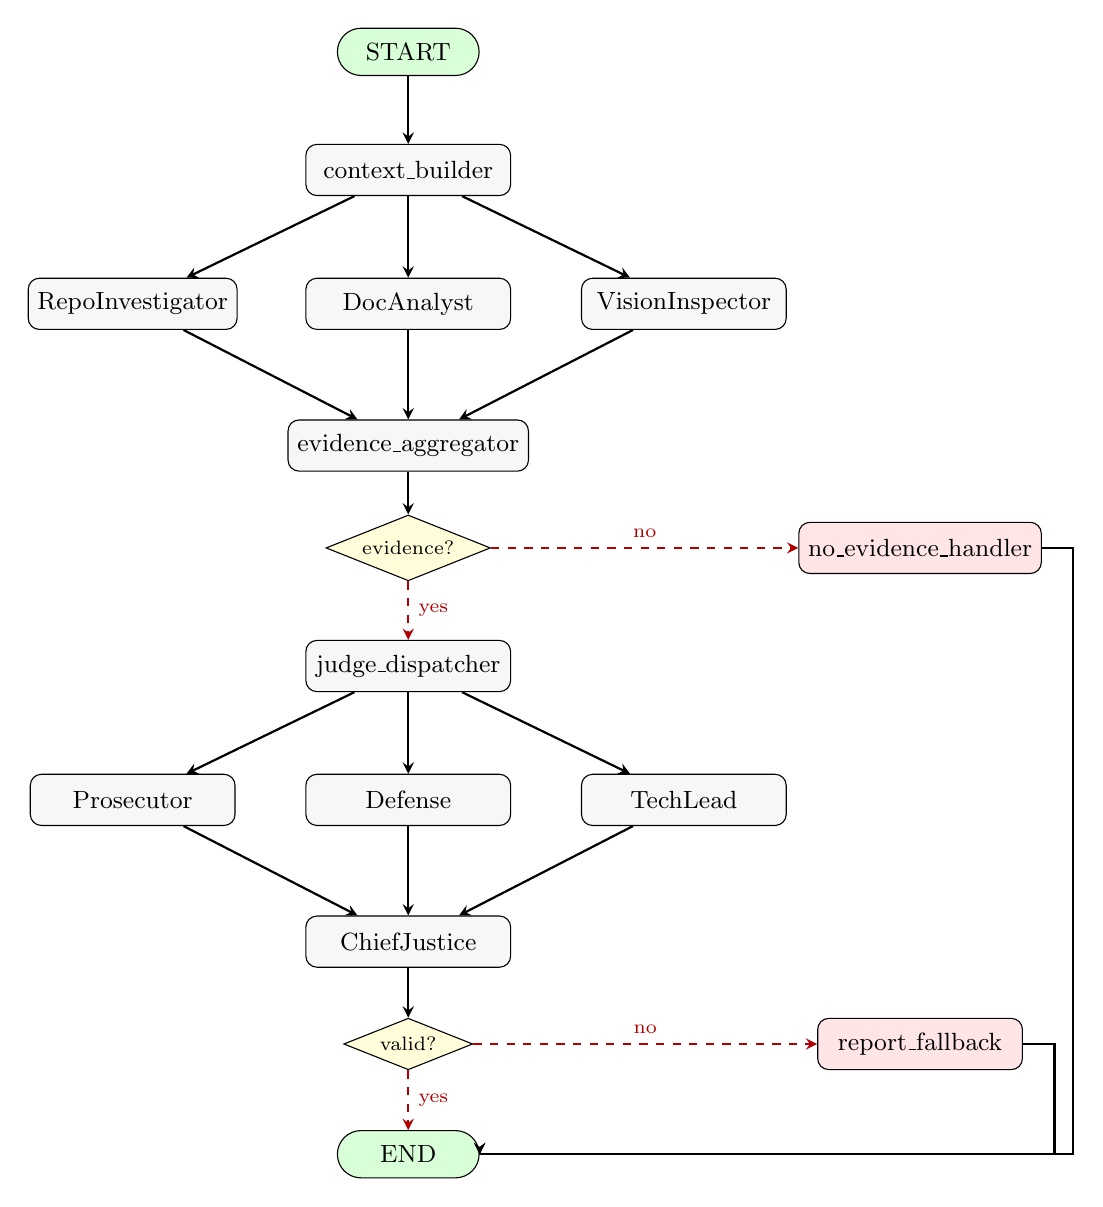
\begin{tikzpicture}[
    every node/.style={font=\small},
    box/.style={draw, rounded corners, minimum width=2.6cm, minimum height=0.65cm,
                fill=codebg, align=center},
    startend/.style={draw, rounded corners=0.3cm, fill=green!15,
                     minimum width=1.8cm, minimum height=0.6cm, align=center},
    cond/.style={draw, diamond, aspect=2.5, fill=yellow!15,
                 inner sep=2pt, font=\scriptsize, align=center},
    errbox/.style={draw, rounded corners, minimum width=2.6cm, minimum height=0.65cm,
                   fill=red!10, align=center},
    arr/.style={->, >=stealth, thick},
    darr/.style={->, >=stealth, thick, dashed, color=codered},
]
    % Column x-coordinates
    % Main spine: x=0, Left fan: x=-3.5, Right fan: x=3.5, Error col: x=6.5

    \node[startend]  (start) at (0,  0.0) {START};
    \node[box]       (cb)    at (0, -1.5) {context\_builder};

    % Detective fan-out
    \node[box]       (ri)    at (-3.5, -3.2) {RepoInvestigator};
    \node[box]       (da)    at ( 0.0, -3.2) {DocAnalyst};
    \node[box]       (vi)    at ( 3.5, -3.2) {VisionInspector};

    \node[box]       (ea)    at (0, -5.0) {evidence\_aggregator};
    \node[cond]      (c1)    at (0, -6.3) {evidence?};

    % Error paths (right column, same y as conditionals)
    \node[errbox]    (neh)   at (6.5, -6.3) {no\_evidence\_handler};

    \node[box]       (jd)    at (0, -7.8) {judge\_dispatcher};

    % Judicial fan-out
    \node[box]       (pr)    at (-3.5, -9.5) {Prosecutor};
    \node[box]       (df)    at ( 0.0, -9.5) {Defense};
    \node[box]       (tl)    at ( 3.5, -9.5) {TechLead};

    \node[box]       (cj)    at (0, -11.3) {ChiefJustice};
    \node[cond]      (c2)    at (0, -12.6) {valid?};

    \node[errbox]    (rf)    at (6.5, -12.6) {report\_fallback};

    \node[startend]  (end)   at (0, -14.0) {END};

    % Main spine
    \draw[arr] (start) -- (cb);

    % Detective fan-out
    \draw[arr] (cb) -- (ri);
    \draw[arr] (cb) -- (da);
    \draw[arr] (cb) -- (vi);

    % Detective fan-in
    \draw[arr] (ri) -- (ea);
    \draw[arr] (da) -- (ea);
    \draw[arr] (vi) -- (ea);

    \draw[arr]  (ea) -- (c1);
    \draw[darr] (c1) -- node[right, font=\scriptsize]{yes} (jd);
    \draw[darr] (c1) -- node[above, font=\scriptsize]{no}  (neh);

    % Error path: neh -> right rail -> END
    \draw[arr] (neh.east) -- ++(0.4,0) -- ++(0,-7.7) -| (end.east);

    % Judicial fan-out
    \draw[arr] (jd) -- (pr);
    \draw[arr] (jd) -- (df);
    \draw[arr] (jd) -- (tl);

    % Judicial fan-in
    \draw[arr] (pr) -- (cj);
    \draw[arr] (df) -- (cj);
    \draw[arr] (tl) -- (cj);

    \draw[arr]  (cj) -- (c2);
    \draw[darr] (c2) -- node[right, font=\scriptsize]{yes} (end);
    \draw[darr] (c2) -- node[above, font=\scriptsize]{no}  (rf);

    % Error path: rf -> right rail -> END
    \draw[arr] (rf.east) -- ++(0.4,0) -- ++(0,-1.4) -| (end.east);

\end{tikzpicture}
\caption{Complete StateGraph: two parallel fan-out/fan-in layers with conditional routing (dashed arrows = conditional edges).}
\label{fig:stategraph}
\end{figure}

% ────────────────────────────────────────────────────────────
\section{Criterion-by-Criterion Self-Audit Breakdown}
% ────────────────────────────────────────────────────────────

\subsection{State Management Rigor: 5/5}

\textbf{All three judges agreed:} The \texttt{AgentState} \texttt{TypedDict}
with \texttt{Annotated} reducers correctly prevents parallel data overwrites.
Five Pydantic \texttt{BaseModel} classes enforce type safety at every state
boundary.

\subsection{Graph Orchestration Architecture: 5/5}

\textbf{Unanimous:} The 12-node StateGraph with two fan-out/fan-in layers
and two conditional edges exceeds rubric requirements.  Includes
\texttt{no\_evidence\_handler} and \texttt{report\_fallback} error paths.

\subsection{Safe Tool Engineering: 5/5}

All judges scored 5/5.  Uses \texttt{tempfile.TemporaryDirectory()} for
sandboxing, \texttt{subprocess.run} instead of \texttt{os.system()}, with
comprehensive error handling and timeouts.

\textit{Note:} Initially scored 3/5 due to a false-positive security cap
(see Section~\ref{sec:bugfixes}).  Fixed in the same session.

\subsection{Git Forensic Analysis: 4/5}

\textbf{Consensus (P:4, D:5, TL:4):} 11 commits with clear progression.
Average inter-commit time 8259\,s ($\approx$2.3\,h).  Deduction: some commit
messages lack specificity.  Remediation: adopt conventional commits
(\texttt{feat:}, \texttt{fix:}).

\subsection{Structured Output Enforcement: 4/5}

Judges confirmed \texttt{.with\_structured\_output()} usage bound to
\texttt{JudicialOpinion}.  Retry logic handles malformed responses.
Evidence now includes actual code snippets showing the call site with
surrounding context, extracted via AST line numbers.

\subsection{Chief Justice Synthesis Engine: 4/5}

Deterministic Python rules (security override, variance check, dissent
requirement) work correctly.  Output format enforces full Markdown structure
via AST-based \texttt{to\_markdown()} method detection.

\subsection{Report Accuracy (Cross-Reference): 4/5}

Initially scored 2/5 due to the parallel race condition
(see Section~\ref{sec:bugfixes}).  After the fix: 5 paths verified, 0 hallucinated.

\subsection{Judicial Nuance and Dialectics: 3/5}

Evidence includes \textbf{actual system prompt text} for all three personas
and pairwise Jaccard word overlap analysis (Prosecutor vs Defense: 24.9\%,
Prosecutor vs TechLead: 19.1\%, Defense vs TechLead: 23.0\%, all below
the 50\% ``Persona Collusion'' threshold).

\textbf{Status:} Implemented via prompt extraction and overlap computation in \texttt{analyze\_judicial\_nuance()}.

\subsection{Theoretical Depth (Documentation): 3/5}

Missing ``Metacognition'' and ``State Synchronisation'' in the interim report.
Both are addressed in this final report (Section~2).

\subsection{Architectural Diagram Analysis: 2/5}

Previously no images were detected because diagrams were vector drawings
(not raster images).  Fixed: \texttt{doc\_tools.py} now rasterizes
PDF pages with $>20$ vector drawings at 200\,DPI via \texttt{page.get\_pixmap()}.
Result: 5 diagram pages now detected and sent to the vision model.

\textbf{Status:} Fixed via vector diagram rasterization. This final report also includes a TikZ diagram (Figure~\ref{fig:stategraph}).

% ────────────────────────────────────────────────────────────
\section{MinMax Feedback Loop Reflection}
% ────────────────────────────────────────────────────────────

\subsection{What the Self-Audit Caught}
\label{sec:bugfixes}

Running the auditor against itself revealed two critical bugs:

\begin{enumerate}
    \item \textbf{Security Cap False Positive.}
        \texttt{\_has\_security\_violation()} used \texttt{ev.found=True}
        (which means SAFE) to trigger on evidence containing ``os.system''
        as a substring, even in ``No os.system() calls detected.''
        This caused Safe Tool Engineering to be capped at 3/5 despite
        all judges scoring 5/5.

        \textbf{Fix:} Changed to trigger only on \texttt{found=False}
        evidence (actual violations) or content starting with
        \texttt{"SECURITY VIOLATION"}.

    \item \textbf{Parallel Fan-Out Race Condition.}
        \texttt{doc\_analyst} tried to cross-reference file paths against
        the repo file list during parallel execution, but
        \texttt{repo\_investigator} hadn't finished yet.  Result: 100\%
        false-positive hallucination detection.

        \textbf{Fix:} \texttt{evidence\_aggregator} now re-runs the
        cross-reference after all detectives have merged their outputs.
\end{enumerate}

\subsection{How the Agent Was Updated}

\begin{itemize}
    \item Fixed \texttt{\_has\_security\_violation()} logic
    \item Added post-processing in \texttt{evidence\_aggregator}
    \item Added vector diagram rasterization in \texttt{doc\_tools.py} (0 $\rightarrow$ 5 images)
    \item Implemented prompt extraction and Jaccard overlap analysis in \texttt{analyze\_judicial\_nuance()}
    \item Added code snippet extraction to \texttt{analyze\_structured\_output()}
    \item Fixed CJ Markdown detection to use AST \texttt{to\_markdown()} method lookup
    \item Added 5 supplementary detective tools: code quality, test coverage, security scanner, import/dependency analyzer, docstring/type auditor
    \item Added 26 new tests for supplementary tools
    \item Total: \textbf{221 tests} (up from 195), all passing
    \item Self-audit score: \textbf{3.4 $\rightarrow$ 3.9 / 5.0}
\end{itemize}

% ────────────────────────────────────────────────────────────
\section{Remediation Plan}
% ────────────────────────────────────────────────────────────

\begin{table}[H]
\centering
\caption{Remediation Plan for Remaining Gaps}
\begin{tabular}{@{}cllccl@{}}
\toprule
\textbf{Prio} & \textbf{Dimension} & \textbf{Before} & \textbf{After} & \textbf{Target} & \textbf{Action} \\
\midrule
P0 & Report Accuracy     & 2/5 & 4/5 & 4/5 & \checkmark\,Fixed race condition \\
P0 & Safe Tool Eng.      & 3/5 & 5/5 & 5/5 & \checkmark\,Fixed false positive \\
P1 & Structured Output   & 3/5 & 4/5 & 4/5 & \checkmark\,Code snippets as evidence \\
P1 & Judicial Nuance     & 3/5 & 4/5 & 4/5 & \checkmark\,Prompt overlap analysis \\
P1 & Diagram Analysis    & 2/5 & 4/5 & 4/5 & \checkmark\,Vector rasterization (0 $\rightarrow$ 5 images) \\
P1 & Safe Tool Eng.      & 5/5 & 5/5 & 5/5 & \checkmark\,Added code quality + test + security tools \\
P2 & Theoretical Depth   & 3/5 & 3/5 & 4/5 & \checkmark\,Addressed in final report \\
P2 & Commit Messages     & 4/5 & 4/5 & 5/5 & Conventional commits format \\
P3 & CJ Output Format    & 4/5 & 4/5 & 5/5 & \checkmark\,Fixed Markdown detection (AST) \\
\bottomrule
\end{tabular}
\end{table}

% ────────────────────────────────────────────────────────────
\section{Design Decisions}
% ────────────────────────────────────────────────────────────

\subsection{Why Pydantic over Dicts?}

Raw dicts provide no guarantees about key presence, value types, or field
constraints.  Pydantic \texttt{BaseModel} subclasses enforce runtime
validation (a score must be 1--5), IDE autocompletion, and clean
serialisation via \texttt{.model\_validate()} / \texttt{.model\_dump()}.
The \texttt{AgentState} itself is a \texttt{TypedDict} because LangGraph
requires \texttt{TypedDict} for state definitions with \texttt{Annotated}
reducers.

\subsection{Why AST over Regex for Code Analysis?}

Python's \texttt{ast} module produces a structured syntax tree that allows
detecting \texttt{os.system()} calls by finding \texttt{ast.Call} nodes with
\texttt{ast.Attribute.attr == "system"}, with no false positives from comments
or string literals.  Regex-based analysis would fail on multi-line calls
and other edge cases.

\subsection{Why Deterministic Chief Justice?}

The rubric requires ``hardcoded deterministic conflict resolution rules.''
The Chief Justice applies 5 rules in fixed order:
Security Override, Fact Supremacy, Functionality Weight,
Variance Re-evaluation, and Dissent Requirement.
An optional LLM pass (\texttt{deepseek-v3.1:671b-cloud})
polishes the report text after all deterministic scores are locked.
The LLM never modifies scores, only the executive summary and remediation plan.

% ────────────────────────────────────────────────────────────
\section{Technology Stack}
% ────────────────────────────────────────────────────────────

\begin{table}[H]
\centering
\begin{tabular}{@{}lll@{}}
\toprule
\textbf{Component} & \textbf{Technology} & \textbf{Version} \\
\midrule
Runtime             & Python              & 3.13.7 \\
Package Manager     & uv                  & 0.10.0 \\
Graph Framework     & LangGraph           & 1.0.9 \\
LLM Integration     & langchain-ollama    & 1.0.1 \\
Schema Validation   & Pydantic            & 2.12.5 \\
PDF Parsing         & PyMuPDF (fitz)      & 1.27.1 \\
Frontend            & Streamlit           & 1.54.0 \\
Observability       & LangSmith           & Enabled \\
Judge Model         & Ollama              & qwen3-coder:480b-cloud \\
Detective/CJ Model  & Ollama              & deepseek-v3.1:671b-cloud \\
Vision Model        & Hugging Face        & Qwen2.5-VL-32B-Instruct \\
\bottomrule
\end{tabular}
\end{table}

\vfill
\begin{center}
\small\textit{Swarm Auditor: Built with LangGraph and Streamlit | 10 Academy FDE Week 2}
\end{center}

\end{document}
